\documentclass[]{scrartcl}
%\usepackage{graphicx}
%\usepackage{amsmath} % For equation alignment
\usepackage{amssymb} % For special math characters such as E with two vertical lines (expectation value symbol)
\usepackage{mathtools} % For some extra math-related functionality, such as matrix*
%\usepackage{hyperref} % For using \autoref
%\usepackage{listings} % For adding code to the latex document
%\usepackage{caption} % For adding captions
\usepackage{color} % For color in code
\usepackage{nicematrix} % For creating matrices with outer rows and columns, with dsahed line separators. Documentation: https://ctan.org/pkg/nicematrix
%\usepackage{float} % For better control over float environments
%\usepackage[utf8]{inputenc} % this is needed for umlauts
%\usepackage[ngerman]{babel} % this is needed for umlauts
%\usepackage[T1]{fontenc}    % this is needed for correct output of umlauts in pdf




% Opening / Title
\title{Complex Systems for Bioinformaticians \\ \vspace{2mm} Assignment 3 \\ \vspace{2mm}}
\subtitle{Lecturers: Prof. Dr. Max von Kleist, Prof. Dr. Jana Wolf, Prof. Dr. Martin Vingron}
\author{Kristian Reinhart, 4474140 \\ Duong Ha Le Minh, 5314209}
\newenvironment{tightcenter}{%
  \setlength\topsep{0pt}
  \setlength\parskip{0pt}
  \begin{center}
}{%
  \end{center}
}




%%%%%%%%%%%%%%%%%%%%%%%%%%%%%%%%%%%
%%%	Begin actual document	%%%
%%%%%%%%%%%%%%%%%%%%%%%%%%%%%%%%%%%


\begin{document}




\maketitle




\section*{3. Assignment}

%%%%%%%%%%%%%%%
%%%	Task 1	%%%
%%%%%%%%%%%%%%%

\subsection*{Task 1)}

Given the weak law of large numbers the standard deviation of the sample mean $\overline{x}^{(p)}$ can be expressed as
$\sigma_{p} ~ = ~ \sqrt{\mathbb{E} \left[ { \vert \overline{x}^{(n)} ~ - ~ \mu \vert }^{2} \right] }$.
\\
The standard deviation $\sigma_{p}$ shrinks at the order of $\mathcal{O} \left( \dfrac{1}{\sqrt{n}} \right)$, with $n$ being the number of samplings.
\\
\\
This in turn means that in order to double the precision (and thus halving the standard deviation $\sigma_{p}$) the number of sampling $n$ must increase by a factor of 4.
Conversely, to halve the precision (and thus doubling the standard deviation $\sigma_{p}$) the number of sampling $n$ must decrease by a factor of 4.
\\
\\
Therefore for the given sample Poisson process with a sample mean  $\sigma_{p}~=~0.05$ for $p~=~1000$ samplings, halving the precision to a sample mean of  $\sigma_{p}~=~0.1$ would require $p~=~250$ samplings. 
\\
\\
\textbf{\textcolor{red}{TODO: Do the derivation for 1 bonus point. Ist this correct?}}
For the derivation we do the following:
\\
\begin{center}
$2* \sigma_{p} ~ = \dfrac{2}{\sqrt{n}}~$
\\
$2* \sigma_{p} ~ = \dfrac{2 * \frac{1}{2}}{\sqrt{n} * \frac{1}{2}}~$
\\
$2* \sigma_{p} ~ = \dfrac{1}{\sqrt{\frac{1}{4} * n}}~$
\end{center}



%%%%%%%%%%%%%%%%%%%
%%%	Task 2a)	%%%
%%%%%%%%%%%%%%%%%%%

\subsection*{Task 2a)}

Given model and reaction rates $r_0$ and $r_1$ we reconstruct the stoichiometric matrix $S$ and rate function vector $R$.

\begin{center}
\noindent \begin{minipage}{.4\linewidth}
$ Model:~ 
\begin{matrix*}[c]
	r_0 & : & x_0 & \rightarrow & x_1 \\
	r_1 & : & x_1 & \rightarrow & \emptyset
\end{matrix*}
$
\end{minipage}
\noindent \begin{minipage}{.4\linewidth}
$
R =
\begin{pNiceMatrix}[last-col,nullify-dots]
	k_a * x_0 & r_0 \\
	k_e	* x_1 & r_1 \\
\end{pNiceMatrix}
$
\end{minipage}
\end{center}

\noindent
From model and reaction rates we reconstruct the stoichiometric matrix $S$:

% Have the matrix in a float-environment and center it, looks nicer
\noindent \begin{center}
\begin{minipage}{.4\linewidth}
$
S =
\begin{pNiceMatrix}[first-row,last-col,nullify-dots]
	R_0	&	R_1 \\
	 -1 &	  0 &	X_0 \\
	  1 &	 -1 &	X_1 \\
\end{pNiceMatrix}
$
\end{minipage}
\end{center}

\noindent 
Finally, combining the stoichiometric matrix $S$ and rate function vector $R$ we can reconstruct the ODE:

\noindent \begin{center}
\begin{minipage}{.5\linewidth}
$
\begin{matrix*}[c]
	\frac{d}{dt} X_0 & = & - & \underbrace{k_a * x_0}	&	& 							\\ 
					 &   &   & 						r_0 &   &							\\
	\frac{d}{dt} X_1 & = &   & \underbrace{k_a * x_0}	& - & \underbrace{k_e * x_1}	\\
					 &   &   & 						r_0 &   &					r_1 
\end{matrix*}
$
\end{minipage}
\end{center}



%%%%%%%%%%%%%%%%%%%
%%%	Task 2b)	%%%
%%%%%%%%%%%%%%%%%%%

%\clearpage
\subsection*{Task 2b)}

\textbf{\textcolor{red}{TODO: Analytically solve the model. Lecture 6, slides 7 and following (3 points)}}



%%%%%%%%%%%%%%%%%%%
%%%	Task 3b)	%%%
%%%%%%%%%%%%%%%%%%%

\clearpage
\subsection*{Task 3b)}

\textbf{\textcolor{red}{TODO: Add plot of 100 simulations}}

\begin{figure}[htbp!]
	\centering
	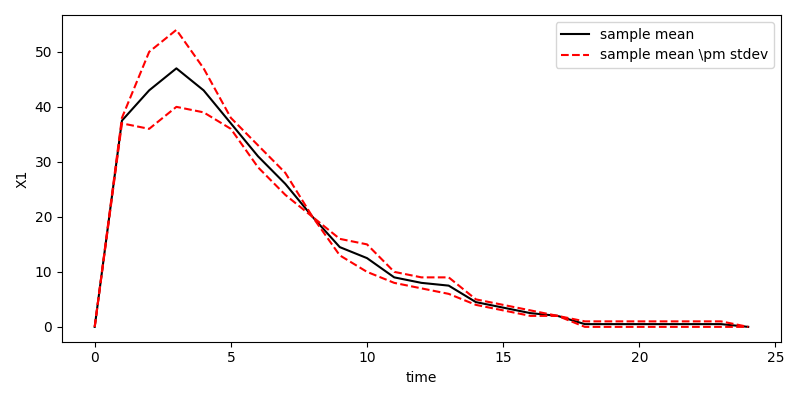
\includegraphics[width=0.6\textwidth]{Exercise3Homework3b.png}
	\caption{100 simulations of the pharmacokinetic model of homework 2.
			 The black line indicates the sample mean $\overline{x}(t)$ and the red dotted lines mark the sample mean $\pm$ one standard deviation.}
\end{figure}



%%%%%%%%%%%%%%%%%%%
%%%	Task 3d)	%%%
%%%%%%%%%%%%%%%%%%%
\clearpage
\subsection*{Task 3d)}

\textbf{\textcolor{red}{TODO: Add plot and discuss order at which error $\epsilon$ tends to zero as a function of $N$, e.g. $\mathcal{O}(?)$}}

\begin{figure}[htbp!]
	\centering
	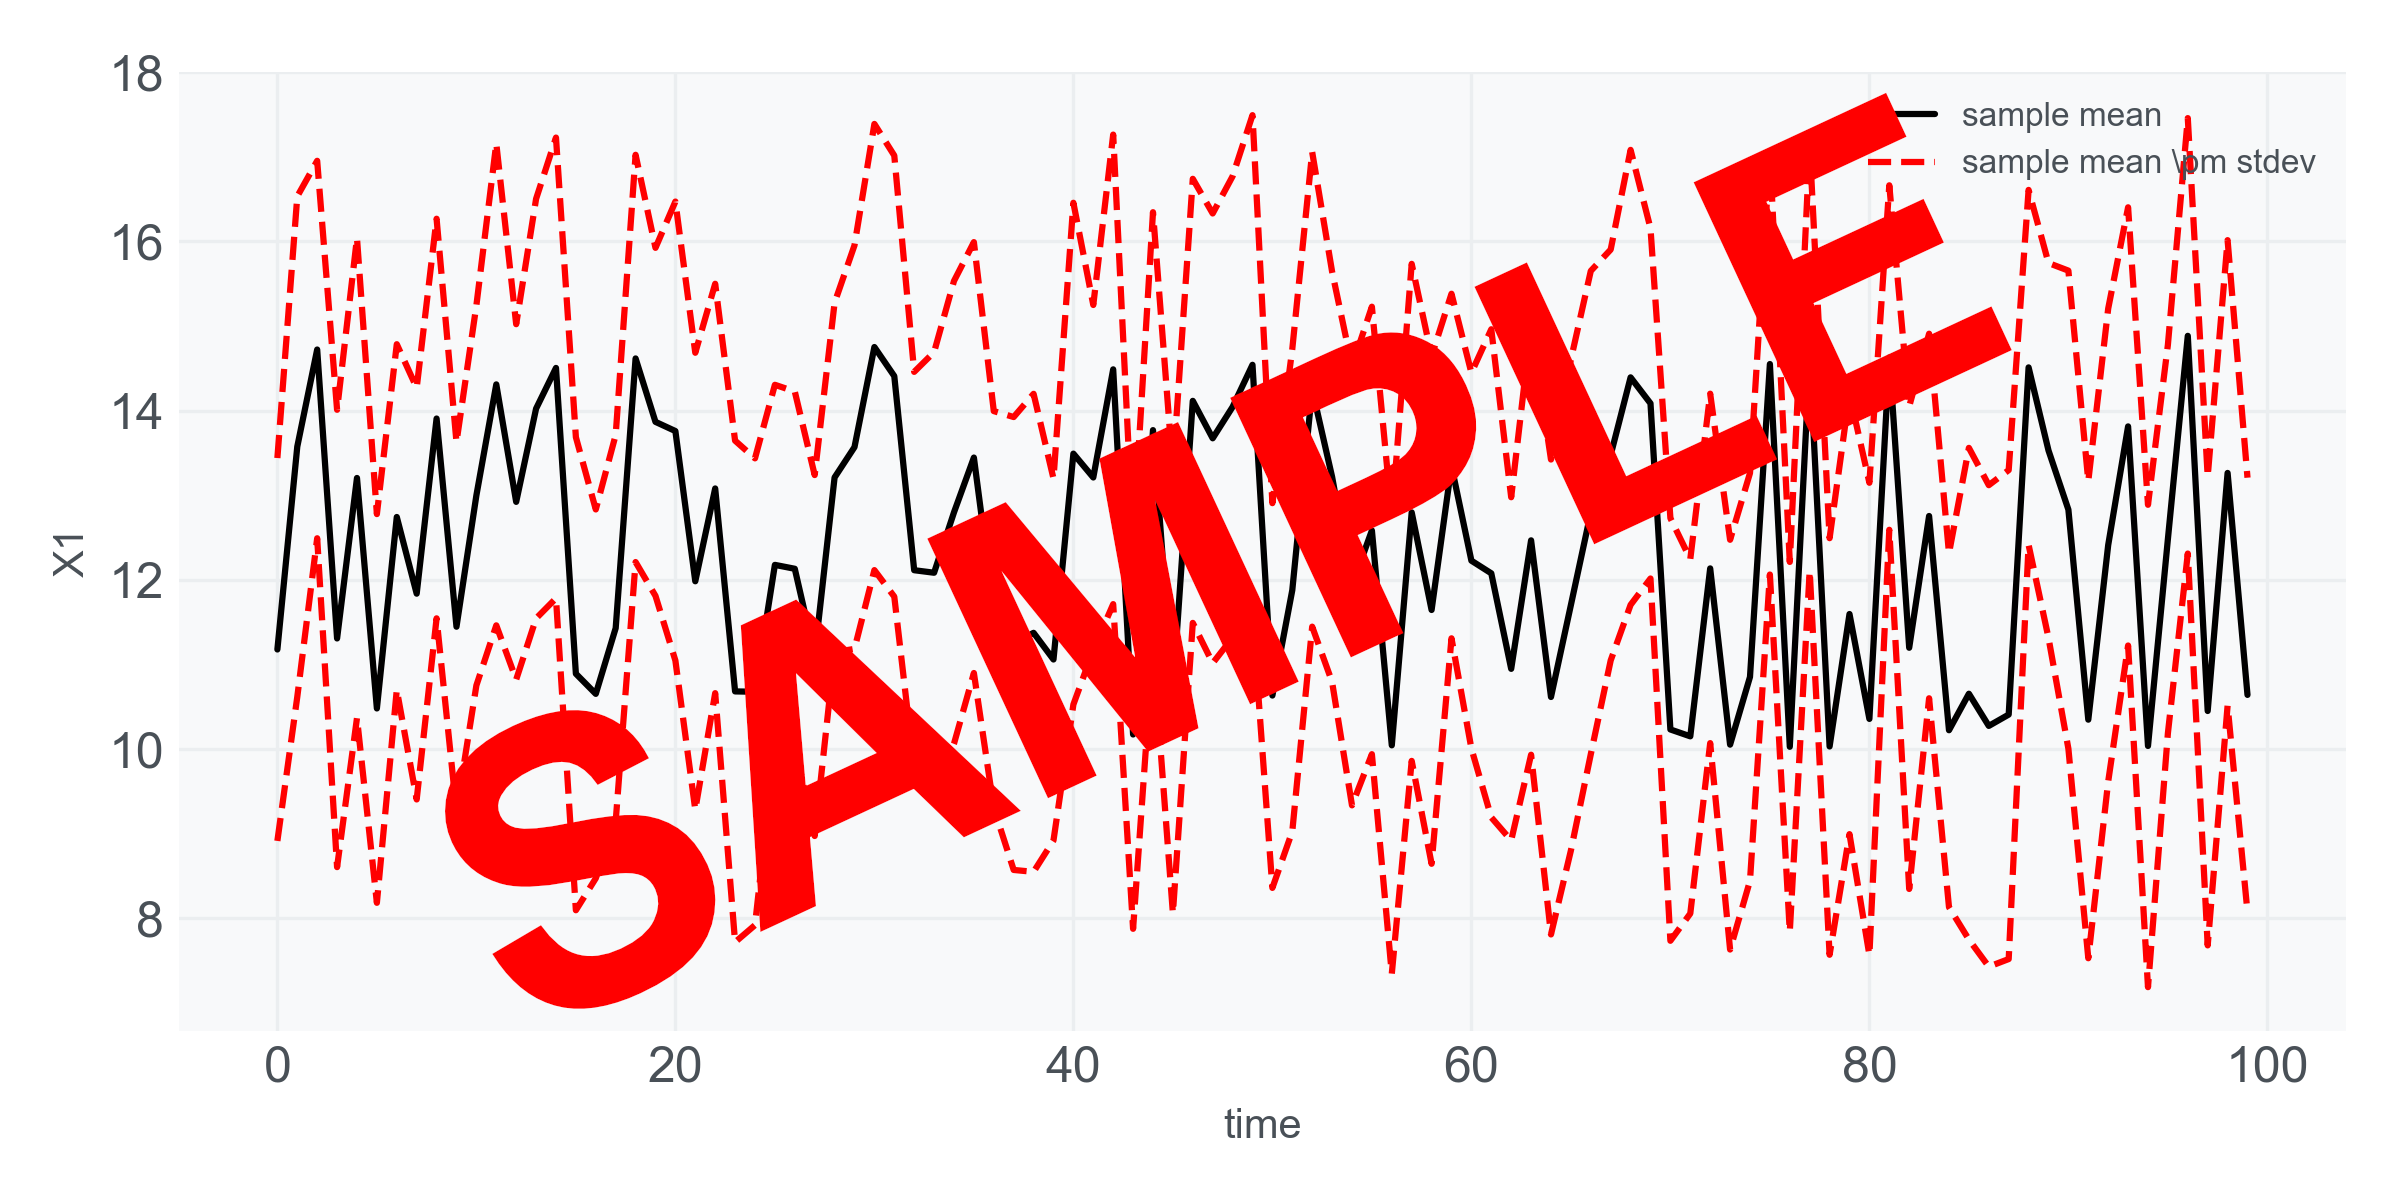
\includegraphics[width=0.6\textwidth]{Exercise3Homework3d.png}
	\caption{ \textbf{\textcolor{red}{TODO: Add caption for plot. Don't know how it'll look, so placeholder.}} }
\end{figure}


\end{document}
